\section{Problem formulation}
Using a swarm $\mathcal{N}$ of $N$ mobile agents with homogenous communication range, we want to deploy them in a mission space, $\Omega$. 
The agents should, without centralized control, spread throughout the mission space and position themselves 
such that they can be used as beacons in a multilateration scheme 
in order to deliver precise positional data to entities entering the mission space.

\subsection{Coverage}\label[secc]{coverage}
It is clear from subsection \ref{trilat} that in two-dimensional space three or more agents are needed to perform the task of multilateration. Hence a point $\mathbf{y}$ is said
to be \textit{covered} iff. the local probability of at least three agents with respect to $\mathbf{y}$ is non-zero. Thus, given a swarm $\mathcal{N}$, the point $\mathbf{y}$ is covered
iff.
\begin{equation}\label[eq]{cover_prob}
  \Phi^{3^{+}}(\mathbf{X}_{\mathcal{N}}, \mathbf{y}) > 0
\end{equation}
We will refer to $\Phi^{3^{+}}(\mathbf{X}_{\mathcal{N}}, \mathbf{y})$ as the probability of coverage.

\subsection{Objective function derivation}\label[secc]{obj_formulation}
The objective function presented here is inspired by \cite{sun2014escaping}, but differs in that for the purpose of multilateration, we apply a stricter definition of coverage (see \ref{coverage}).

In order to formulate a distributed optimization algorithm, we rewrite the probability of coverage with focus on a single drone $a$.
Using \eqref{more_than_n_prob} we can write the probability of coverage \eqref{cover_prob} as:
\begin{equation}
  \Phi^{3^{+}}(\mathbf{X}_{\mathcal{N}}, \mathbf{y}) = 1 - \Phi^{2}(\mathbf{X}_{\mathcal{N}}, \mathbf{y}) - \Phi^{1}(\mathbf{X}_{\mathcal{N}}, \mathbf{y}) - \Phi^{0}(\mathbf{X}_{\mathcal{N}}, \mathbf{y})
\end{equation}
We partition the swarm, $\mathcal{N}$, into two disjoint sets: $\{a\}$ and $\mathcal{N}\setminus\{a\}$. Using this we can rewrite \eqref{cover_prob} as:
\begin{equation}\label[eq]{distr_cover_derivation}
  \begin{split}
    \Phi^{3^{+}}(\mathbf{X}_{\mathcal{N}}, \mathbf{y}) &= 1\\
    &- \big(1-\hat{p}(\mathbf{x}_{a}, \mathbf{y})\big)\prod_{k\in\mathcal{N}\setminus\{a\}}\big(1-\hat{p}(\mathbf{x}_{k}, \mathbf{y}))\\
    &- \hat{p}(\mathbf{x}_{a}, \mathbf{y})\prod_{k\in\mathcal{N}\setminus\{a\}}\big(1-\hat{p}(\mathbf{x}_{k}, \mathbf{y}))\\
    &- \big(1-\hat{p}(\mathbf{x}_{a}, \mathbf{y})\big)\sum_{j\in\mathcal{N}\setminus\{a\}}\hat{p}(\mathbf{x}_{j}, \mathbf{y})\prod_{k\in\mathcal{N}\setminus\{a\}\setminus\{j\}}\big(1-\hat{p}(\mathbf{x}_{k}, \mathbf{y})\big)\\
    &- \hat{p}(\mathbf{x}_{a}, \mathbf{y})\sum_{j\in \mathcal{N}\setminus\{a\}}\hat{p}(\mathbf{x}_{j}, \mathbf{y})\prod_{k\in\mathcal{N}\setminus\{a\}\setminus\{j\}}\big(1-\hat{p}(\mathbf{x}_{k}, \mathbf{y})\big)\\
    &- \big(1-\hat{p}(\mathbf{x}_{a}, \mathbf{y})\big)\sum_{\mathcal{A}\in Comb(\mathcal{N}\setminus\{a\}, 2)}\prod_{j\in\mathcal{A}}\hat{p}(\mathbf{x}_{j}, \mathbf{y})\prod_{k\in\mathcal{N}\setminus\{a\}\setminus\mathcal{A}}\big(1-\hat{p}(\mathbf{x}_{k}, \mathbf{y})\big)\\
    &= 1\\
    &- \prod_{k\in\mathcal{N}\setminus\{a\}}\big(1-\hat{p}(\mathbf{x}_{k}, \mathbf{y}))\\
    &- \sum_{j\in\mathcal{N}\setminus\{a\}}\hat{p}(\mathbf{x}_{j}, \mathbf{y})\prod_{k\in\mathcal{N}\setminus\{a\}\setminus\{j\}}\big(1-\hat{p}(\mathbf{x}_{k}, \mathbf{y})\big)\\
    &- \big(1-\hat{p}(\mathbf{x}_{a}, \mathbf{y})\big)\sum_{\mathcal{A}\in Comb(\mathcal{N}\setminus\{a\}, 2)}\prod_{j\in\mathcal{A}}\hat{p}(\mathbf{x}_{j}, \mathbf{y})\prod_{k\in\mathcal{N}\setminus\{a\}\setminus\mathcal{A}}\big(1-\hat{p}(\mathbf{x}_{k}, \mathbf{y})\big)\\
  \end{split}
\end{equation}
Applying \eqref{Phi_def} to \eqref{distr_cover_derivation} yields:
\begin{equation}\label[eq]{local_coverage}
  \begin{split}
    \Phi^{3^{+}}(\mathbf{X}_{\mathcal{N}}, \mathbf{y}) &= 1 - \Phi^{0}(\mathbf{X}_{\mathcal{N}\setminus\{a\}}, \mathbf{y}) - \Phi^{1}(\mathbf{X}_{\mathcal{N}\setminus\{a\}}, \mathbf{y}) - \Phi^{2}(\mathbf{X}_{\mathcal{N}\setminus\{a\}}, \mathbf{y})\big(1-\hat{p}(\mathbf{x}_{a}, \mathbf{y})\big)\\
    &= \Phi^{3^{+}}(\mathbf{X}_{\mathcal{N}\setminus\{a\}}, \mathbf{y}) + \Phi^{2}(\mathbf{X}_{\mathcal{N}\setminus\{a\}}, \mathbf{y})\hat{p}(\mathbf{x}_{a}, \mathbf{y})\\
  \end{split}
\end{equation}
Rewriting \eqref{local_coverage} yields:
\begin{equation}
  \begin{split}
    \Phi^{3^{+}}(\mathbf{X}_{\mathcal{N}}, \mathbf{y}) &= \Phi^{3^{+}}(\mathbf{X}_{\mathcal{N}\setminus\{a\}}, \mathbf{y}) - \hat{p}(\mathbf{x}_{a}, \mathbf{y})\Phi^{3^{+}}(\mathbf{X}_{\mathcal{N}\setminus\{a\}}, \mathbf{y}) + \hat{p}(\mathbf{x}_{a}, \mathbf{y})\Phi^{2^{+}}(\mathbf{X}_{\mathcal{N}\setminus\{a\}}, \mathbf{y})\\
    &= (1-\hat{p}(\mathbf{x}_{a}, \mathbf{y}))\Phi^{3^{+}}(\mathbf{X}_{\mathcal{N}\setminus\{a\}}, \mathbf{y}) + \hat{p}(\mathbf{x}_{a}, \mathbf{y})\Phi^{2^{+}}(\mathbf{X}_{\mathcal{N}\setminus\{a\}}, \mathbf{y})\\
  \end{split}
\end{equation}
It is clear that the probability of the point $\mathbf{y}$ being covered can be seen on as an interpolation between two probability measures with the local probability of agent $a$ as the interpolation variable. Low local probability of agent $a$ means that the probability of coverage supplied the swarm as a whole depends more on the coverage supplied by
the swarm excluding agent $a$. In the extreme case where the local probability of agent $a$ is zero, the probability of covering $\mathbf{y}$ depends only on the coverage supplied by the swarm excluding agent $a$.

Higher local probability of agent $a$ means that the contribution of $a$ towards covering the point $\mathbf{y}$ is greater, thus less weight is put on the the probability of the swarm excluding agent $a$ covering the point. Instead more weight is put on the probability of at least \textit{two} other agents being able to communicate with an entity at $\mathbf{y}$. 
This is due to the fact that the probability of agent $a$ being able to communicate with said entity is higher, and we need only two or more other agents to be able to communicate with the entity at $\mathbf{y}$ to make the total number of agents covering $\mathbf{y}$ three or more.

\begin{figure}[H]
  \centering
  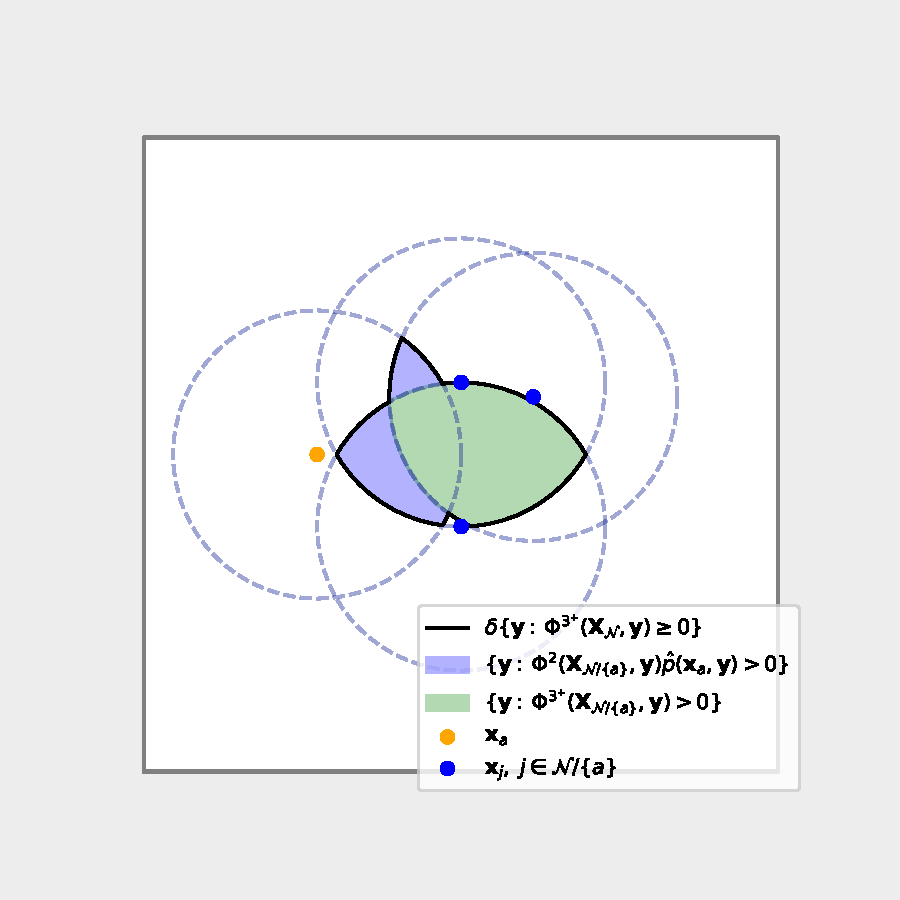
\includegraphics[width=.75\textwidth]{figs/local_objective_example.pdf}
  \caption{Non-zero regions of integrands in \eqref{rewritten_objective}. Note that perturbing the orange circle (position of agent $a$) does not affect the green region,
  as it is defined only by the intersections of the disks surrounding the blue points (other agents in the swarm).}
  \label[fig]{local_coverage_example}
\end{figure}

We note that the overall probability of coverage over the feasible space can be written as:
\begin{equation}\label[eq]{rewritten_objective}
  \begin{split}
    P(\mathbf{X}_{\mathcal{N}}) &=\int_{\mathcal{F}}\Phi^{3^{+}}(\mathbf{X}_{\mathcal{N}}, \mathbf{y})d\mathbf{y} =  \int_{\mathcal{F}}\Phi^{3^{+}}(\mathbf{X}_{\mathcal{N}\setminus\{a\}}, \mathbf{y}) + \Phi^{2}(\mathbf{X}_{\mathcal{N}\setminus\{a\}}, \mathbf{y})\hat{p}(\mathbf{x}_{a}, \mathbf{y})d\mathbf{y}\\
    &= \int_{\mathcal{F}}\Phi^{3^{+}}(\mathbf{X}_{\mathcal{N}\setminus\{a\}}, \mathbf{y})d\mathbf{y} + \int_{\mathcal{F}}\Phi^{2}(\mathbf{X}_{\mathcal{N}\setminus\{a\}}, \mathbf{y})\hat{p}(\mathbf{x}_{a}, \mathbf{y})d\mathbf{y}\\
  \end{split}
\end{equation}
The first term in \eqref{rewritten_objective} is independent of the position of $a$ in both its domain and integrand. This independence is visualized in \figref{local_coverage_example}. Thus we can rewrite the overall coverage probability over $\mathcal{F}$ as:
\begin{equation}
  P(\mathbf{X}_{\mathcal{N}}) = P(\mathbf{X}_{\mathcal{N}\setminus\{a\}}) + P_{a}(\mathbf{X}_{\mathcal{N}})
\end{equation}
Where the \textit{local} probability of coverage for agent $a$ is defined as:
\begin{equation}\label[eq]{local_objective}
  P_{a}(\mathbf{X}_{\mathcal{N}}) = \int_{\mathcal{F}}\Phi^{2}(\mathbf{X}_{\mathcal{N}\setminus\{a\}}, \mathbf{y})\hat{p}(\mathbf{x}_{a}, \mathbf{y})d\mathbf{y}
\end{equation}

As in \cite{sun2014escaping} we note that from the viewpoint of agent $a$, the swarm can be partitioned into three disjoint sets: $\{a\}$, $\mathcal{B}_{a}$ and $\mathcal{C}_{a}$. 
Exploiting that all agents have homogenous range of communication, i.e.
\begin{equation}
  r_{a} = r\;\forall\:a\in\mathcal{N}
\end{equation}
we define
\begin{subequations}\label[eq]{B_a_and_C_a_def}
  \begin{equation}\label[eq]{neigh_def}
    \mathcal{B}_{a} = \{j\in\mathcal{N}\setminus\{a\}: \norm{\mathbf{x}_{a}-\mathbf{x}_{j}} \leq 2r\}
  \end{equation}
  \begin{equation}
    \mathcal{C}_{a} = \{j\in\mathcal{N}\setminus\{a\}: \norm{\mathbf{x}_{a}-\mathbf{x}_{j}} > 2r\}
  \end{equation}  
\end{subequations}
The set $\mathcal{B}_{a}$, from now on called the neighbors of $a$, contains all agents in the swarm, $\mathcal{N}$, whose communication disks form a non-empty intersection with that of $a$.
$\mathcal{C}_{a}$ contains all agents whose communication disks do not intersect with that of $a$.

Applying \eqref{B_a_and_C_a_def} to \eqref{local_objective} yields:
\begin{equation}
  \begin{split}
    P_{a}(\mathbf{X}_{\mathcal{N}}) &= \int_{\mathcal{F}}\Phi^{2}(\mathbf{X}_{\mathcal{N}\setminus\{a\}}, \mathbf{y})\hat{p}(\mathbf{x}_{a}, \mathbf{y})d\mathbf{y}\\
    &= \int_{\mathcal{F}}\Big(\Phi^{2}(\mathbf{X}_{\mathcal{B}_{a}}, \mathbf{y}) + \Phi^{2}(\mathbf{X}_{\mathcal{C}_{a}}, \mathbf{y}) + \Phi^{1}(\mathbf{X}_{\mathcal{B}_{a}}, \mathbf{y})\Phi^{1}(\mathbf{X}_{\mathcal{C}_{a}}, \mathbf{y})\Big)\hat{p}(\mathbf{x}_{a}, \mathbf{y})d\mathbf{y}
  \end{split}
\end{equation}
Partitioning the domain of integration into the visible set and invisible set of agent $a$, and noting that $\hat{p}(\mathbf{x}_{j}, \mathbf{y}) = 0\;\forall\;j\in\mathcal{C}_{a},\;\mathbf{y}\in V_{a}$ such that
$\Phi^{n}(\mathbf{X}_{\mathcal{C}_{a}}, \mathbf{y}) = 0\;\forall\;n\in\mathbb{Z}^{+},\;\mathbf{y}\in V_{a}$, and $\hat{p}(\mathbf{x}_{a}, \mathbf{y}) = 0\;\forall\;\mathbf{y}\in U_{a}$ yields:
\begin{equation}\label[eq]{local_objective_derivated}
  \begin{split}
    P_{a}(\mathbf{X}_{\mathcal{N}}) &= \int_{V_{a}}\Big(\Phi^{2}(\mathbf{X}_{\mathcal{B}_{a}}, \mathbf{y}) + \Phi^{2}(\mathbf{X}_{\mathcal{C}_{a}}, \mathbf{y}) + \Phi^{1}(\mathbf{X}_{\mathcal{B}_{a}}, \mathbf{y})\Phi^{1}(\mathbf{X}_{\mathcal{C}_{a}}, \mathbf{y})\Big)\hat{p}(\mathbf{x}_{a}, \mathbf{y})d\mathbf{y}\\
    &+ \int_{U_{a}}\Big(\Phi^{2}(\mathbf{X}_{\mathcal{B}_{a}}, \mathbf{y}) + \Phi^{2}(\mathbf{X}_{\mathcal{C}_{a}}, \mathbf{y}) + \Phi^{1}(\mathbf{X}_{\mathcal{B}_{a}}, \mathbf{y})\Phi^{1}(\mathbf{X}_{\mathcal{C}_{a}}, \mathbf{y})\Big)\hat{p}(\mathbf{x}_{a}, \mathbf{y})d\mathbf{y}\\
    &= \int_{V_{a}}\Phi^{2}(\mathbf{X}_{\mathcal{B}_{a}}, \mathbf{y})p(\norm{\mathbf{x}_{a}-\mathbf{y}})d\mathbf{y} = L(\mathbf{X}_{\mathcal{B}_{a}\cup\{a\}})
  \end{split}
\end{equation}
Thus the local probability of coverage for an agent $a$ is dependent on the position, $\mathbf{x}_{a}$, of agent $a$ in both domain and integrand, and the positions of the neighbors of agent $a$.
We call the swarm consisting of $a$ and its neighbors agent $a$'s local swarm.\clearpage

As discussed in subsection \ref{trilat} it is beneficial that agents used for multilateration spread out to some extent in order to ensure sufficient accuracy of multilateration.
Furthermore ensuring that agents spread throughout the mission space is desirable.
In order to encourage spread of agents we introduce a term penalizing an agent $a$ for being close to another agent $j$. 
When agents are close to each other we want this term to induce some velocity in the agents causing
them to spread.
In \cite{pot_field} virtual potential fields are used to disperse agents. The potential between an agent $a$ and its neighbor $j$ is modelled as:
\begin{equation}\label[eq]{pt_field}
  U = -k\frac{1}{\norm{\mathbf{x}_{a} - \mathbf{x}_{j}}}
\end{equation}
where $k$ is a constant defining the strength of the field.
Drawing inspiration from this we propose the proximity term between two agents $a$ and $j$:
\begin{equation}\label[eq]{proximity_func}
  D(\mathbf{x}_{a}, \mathbf{x}_{j}) = k_{1}e^{-k_{2}\norm{\mathbf{x}_{a} - \mathbf{x}_{j}}}
\end{equation}
We note that as opposed to \eqref{pt_field}, \eqref{proximity_func} is defined for all $\mathbf{x}_{a},\:\mathbf{x}_{j}$ allowing for easier implementation. The function has two tunable parameters, $k_{1},\:k_{2}\geq 0$, whose effects are show in \figref{cdr}.

Using \eqref{local_objective_derivated} and \eqref{proximity_func}  We now state the \textit{local} objective for an agent $a$ as:
\begin{equation}\label[eq]{local_objective_func}
  H(\mathbf{X}_{\mathcal{B}_{a}\cup\{a\}})  = L(\mathbf{X}_{\mathcal{B}_{a}\cup\{a\}})  - \sum_{j\in\mathcal{B}_{a}}D(\mathbf{x}_{a}, \mathbf{x}_{j})
\end{equation}
Due to the negative sign in front of the sum of proximity functions, we will refer to this as the active dispersion term.
\begin{figure}[H]
  \centering
  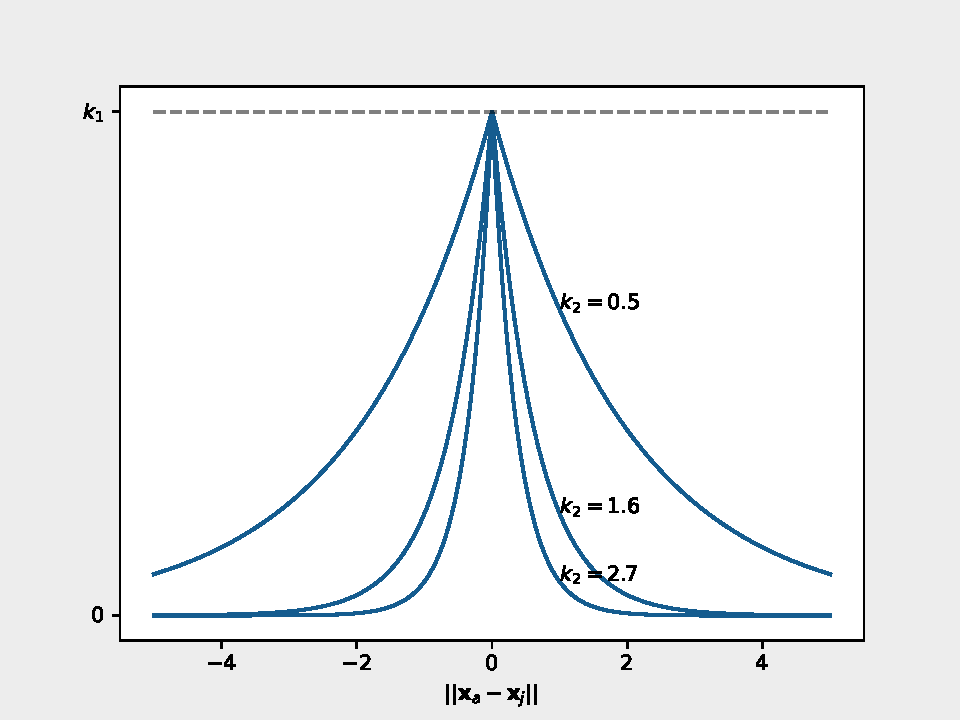
\includegraphics[width=.7\textwidth]{figs/close_dist_repell_example.pdf}
  \caption{Proximity term in \eqref{proximity_func} for an agent, $a$, and its neighbor, $j$.}
  \label[fig]{cdr}
\end{figure}

\subsection{Constraints}\label[secc]{constraints}
It is clear from subsection \ref{trilat} that agents used as beacons in a multilateration scheme cannot be positioned on a straight line, as this would make it impossible
to uniquely determine the unknown position of an entity. Due to the fact that only agents close to the entity whose position is to be determined will
take part in the multilateration scheme, we impose only that agents that together can be used for multilateration must satisfy the non-linear position requirement.

For an agent $a$ with $N$ neighbors $j\in\mathcal{B}_{a},\:|B_{a}|=N$ we construct a matrix $\mathbf{V}$ according to:
\begin{equation}\label[eq]{V_def}
  \mathbf{V}(\mathbf{X}_{\mathcal{B}_{a}}) = \begin{bmatrix}
    \mathbf{X}_{\mathcal{B}_{a, 0}}-\mathbf{X}_{\mathcal{B}_{a, 1}}&\hdots&\mathbf{X}_{\mathcal{B}_{a, 0}}-\mathbf{X}_{\mathcal{B}_{a, N-1}}.
  \end{bmatrix}
\end{equation}
If agent $a$ has less than two neighbors, or all of agent $a$'s neighbors are positioned on a straight line, the matrix $\mathbf{V}(\mathbf{X}_{\mathcal{B}_{a}})$ will not span $\mathbb{R}^{2}$, i.e. $\mathrm{Rank}(\mathbf{V}(\mathbf{X}_{\mathcal{B}_{a}})) < 2$.

Assuming that agent $a$ has two or more neighbors, $|\mathcal{B}_{a}|\geq 2$, and that all neighbors of $a$ are positioned on a straight line, it is desirable that agent $a$ is positioned sufficiently far away from the line. This constraint is implemented as follows:
Without loss of generality we define:
\begin{subequations}\label[eq]{vl}
  \begin{align}
    \mathbf{v}(\mathbf{x}_{a}) &= \mathbf{x}_{a} - \mathbf{X}_{\mathcal{B}_{a}, 0}\\
    \mathbf{l} &= \mathbf{X}_{\mathcal{B}_{a}, 1} - \mathbf{X}_{\mathcal{B}_{a}, 0},
  \end{align}
\end{subequations}
meaning $\mathbf{v}(\mathbf{x}_{a})$ is the vector from agent $a$ to its first neighbor, and $\mathbf{l}$ is the vector between agent $a$'s first and second neighbor. Thus $\mathbf{l}$ is parallel to the line 
that goes through all of agent $a$'s neighbors.
Using (3.98) in \cite{projection} to project $\mathbf{v}(\mathbf{x}_{a})$ into $\mathbf{l}$ we get the component of $\mathbf{v}(\mathbf{x}_{a})$ that is parallel to the line
through agent $a$'s neighbor $i$ and $j$:
\begin{equation}
  \mathbf{v}_{\parallel}(\mathbf{x}_{a}) = \frac{\mathbf{v}(\mathbf{x}_{a})^{T}\mathbf{l}}{\mathbf{l}^{T}\mathbf{l}}\mathbf{l}
\end{equation}
The component of $\mathbf{v}(\mathbf{x}_{a})$ perpendicular to the line through agent $a$'s
neighbors is obtained as:
\begin{equation}
  \mathbf{v}_{\perp}(\mathbf{x}_{a}) = \mathbf{v}(\mathbf{x}_{a}) - \mathbf{v}_{\parallel}(\mathbf{x}_{a})
\end{equation}
Now the distance from agent $a$ to the line through its neighbors can be computed as:
\begin{equation}
  \norm{\mathbf{v}_{\perp}(\mathbf{x}_{a})} = \norm{\mathbf{v}(\mathbf{x}_{a}) - \frac{\mathbf{v}(\mathbf{x}_{a})^{T}\mathbf{l}}{\mathbf{l}^{T}\mathbf{l}}\mathbf{l}}
\end{equation}
Seen as it is impossible to place and agent such that it lays on a straight line through all it's neighbors if the neighbors do not already
lay on a straight line we demand that the non-linear position constraint be fulfilled only when $\mathrm{Rank}(\mathbf{V}(\mathbf{X}_{\mathcal{B}_{a})}) < 2$, where $\mathbf{V}(\cdot)$ is defined in \eqref{V_def}. The non-linear position constraint is defined as:
\begin{equation}\label[eq]{non_lin_pos}
    \norm{\mathbf{v}(\mathbf{x}_{a}) - \frac{\mathbf{v}(\mathbf{x}_{a})^{T}\mathbf{l}}{\mathbf{l}^{T}\mathbf{l}}\mathbf{l}}\geq d_{min} 
\end{equation}
where $d_{min}$ is a tunable parameter that defines how close an agent is allowed get to the line through it's neighbors, and $\mathbf{v}$ and $\mathbf{l}$
are defined in \eqref{vl}.

We also impose that any two agents must be some minimum distance apart at any given time. This is due to the fact that agents colliding could cause damage to the hardware, and possibly render them unusable.
This constraint is modelled as:
\begin{equation}
  \norm{\mathbf{x}_{a} - \mathbf{x}_{j}} \geq r_{min} \;\forall\;j\in\mathcal{B}_{a},
\end{equation}
where $r_{min}$ is a tunable parameter that sets a limit to how close an agent can be positioned to any of its neighbors.\clearpage
\subsection{Optimization problem formulation}
The non-linear position constraint \eqref{non_lin_pos} presented in \ref{constraints} is dependent on the neighbor set of agent $a$, $\mathcal{B}_{a}$, as it should only be imposed if the 
neighbors of agent $a$ lay on a straight line. Using the objective function in \eqref{local_objective_func} and the constraints in discussed in \ref{constraints} we define the optimization problem:
\begin{subequations}\label[eq]{local_opt_prob}
  \begin{align}
    \begin{split}\label[eq]{totally_objective}
      &\max_{\mathbf{x}_{a}}\;H(\mathbf{X}_{\mathcal{B}_{a}\cup\{a\}})\\
    \end{split}\\
    \mathrm{s.t.}\;
    \begin{split}
      &\mathbf{x}_{a}\in\mathcal{F}
    \end{split}\\
    \begin{split}\label[eq]{min_two_neig}
      &|\{j\in\mathcal{B}_{a}: \norm{\mathbf{x}_{a} - \mathbf{x}_{j}} \leq 2r\}|\geq 2
    \end{split}\\
    \begin{split}\label[eq]{min_dist_neigh}
      &\norm{\mathbf{x}_{a} - \mathbf{x}_{j}} \geq r_{min}\;\forall\;j\in\mathcal{B}_{a}
    \end{split}\\
    \begin{split}\label[eq]{non_linear_neighb}
      &\norm{\mathbf{v}(\mathbf{x}_{a}) - \frac{\mathbf{v}(\mathbf{x}_{a})^{T}\mathbf{l}}{\mathbf{l}^{T}\mathbf{l}}\mathbf{l}}\geq d_{min},\quad\mathrm{iff.}\;\mathrm{Rank}(\mathbf{V}(\mathbf{X}_{\mathcal{B}_{a}}))<2
    \end{split}
\end{align}
\end{subequations}
where $\mathbf{V}(\cdot)$ is defined in \eqref{V_def} and $\mathbf{v}(\cdot)$ and $\mathbf{l}$ are defined in \eqref{vl}.

In situations where $\frac{\partial L(\mathbf{X}_{\mathcal{B}_{a}\cup\{a\}})}{\partial \mathbf{x}_{a}} = 0$ the solution of \eqref{totally_objective} will be achieved at the position $\mathbf{x}_{a}$ that minimizes the dispersion term in \eqref{local_objective_func}.
This will cause agent $a$ to move as far away from its neighbors as possible. Such behavior is undesirable as this might render agent $a$ neighbor-less. For an agent 
$a$ without neighbors we have $\mathcal{B}_{a} = \emptyset$ and hence $H(\mathbf{X}_{\mathcal{B}_{a}\cup\{a\}}) \equiv 0$. Thus re-optimization will result in $\mathbf{x}_{a}$ being unaltered, causing agent $a$
to stay at $\mathbf{x}_{a}$ indefinitely. To prevent such behavior we impose the constraint \eqref{min_two_neig}. This will prevent agent $a$ from completely disconnecting from its local swarm. 

Furthermore we observe that Rank$(\mathbf{V}(\mathbf{X}_{\mathcal{B}_{a}}))<2$ if either all neighbors of agent $a$ lie on a straight line or agent $a$ has less than two neighbors. If agent $a$ has less than
two neighbors it is not possible to draw a line between the neighbors of agent $a$, and thus the non-linear neighbor constraint \eqref{non_linear_neighb} is undefined. This further motivates imposing the constraint that
agent $a$ should have at least two neighbors at the solution to \eqref{local_opt_prob}.

The optimization problem formulated in \eqref{local_opt_prob} is non-convex \cite{NoceWrig06_convex_prob}. The objective function is generally non-concave and the constraints form a non-convex feasible set. In 
\figref{objective_example} a visualization of the objective function is shown for an agent with 5 neighbors.
\begin{figure}[H]
  \centering
  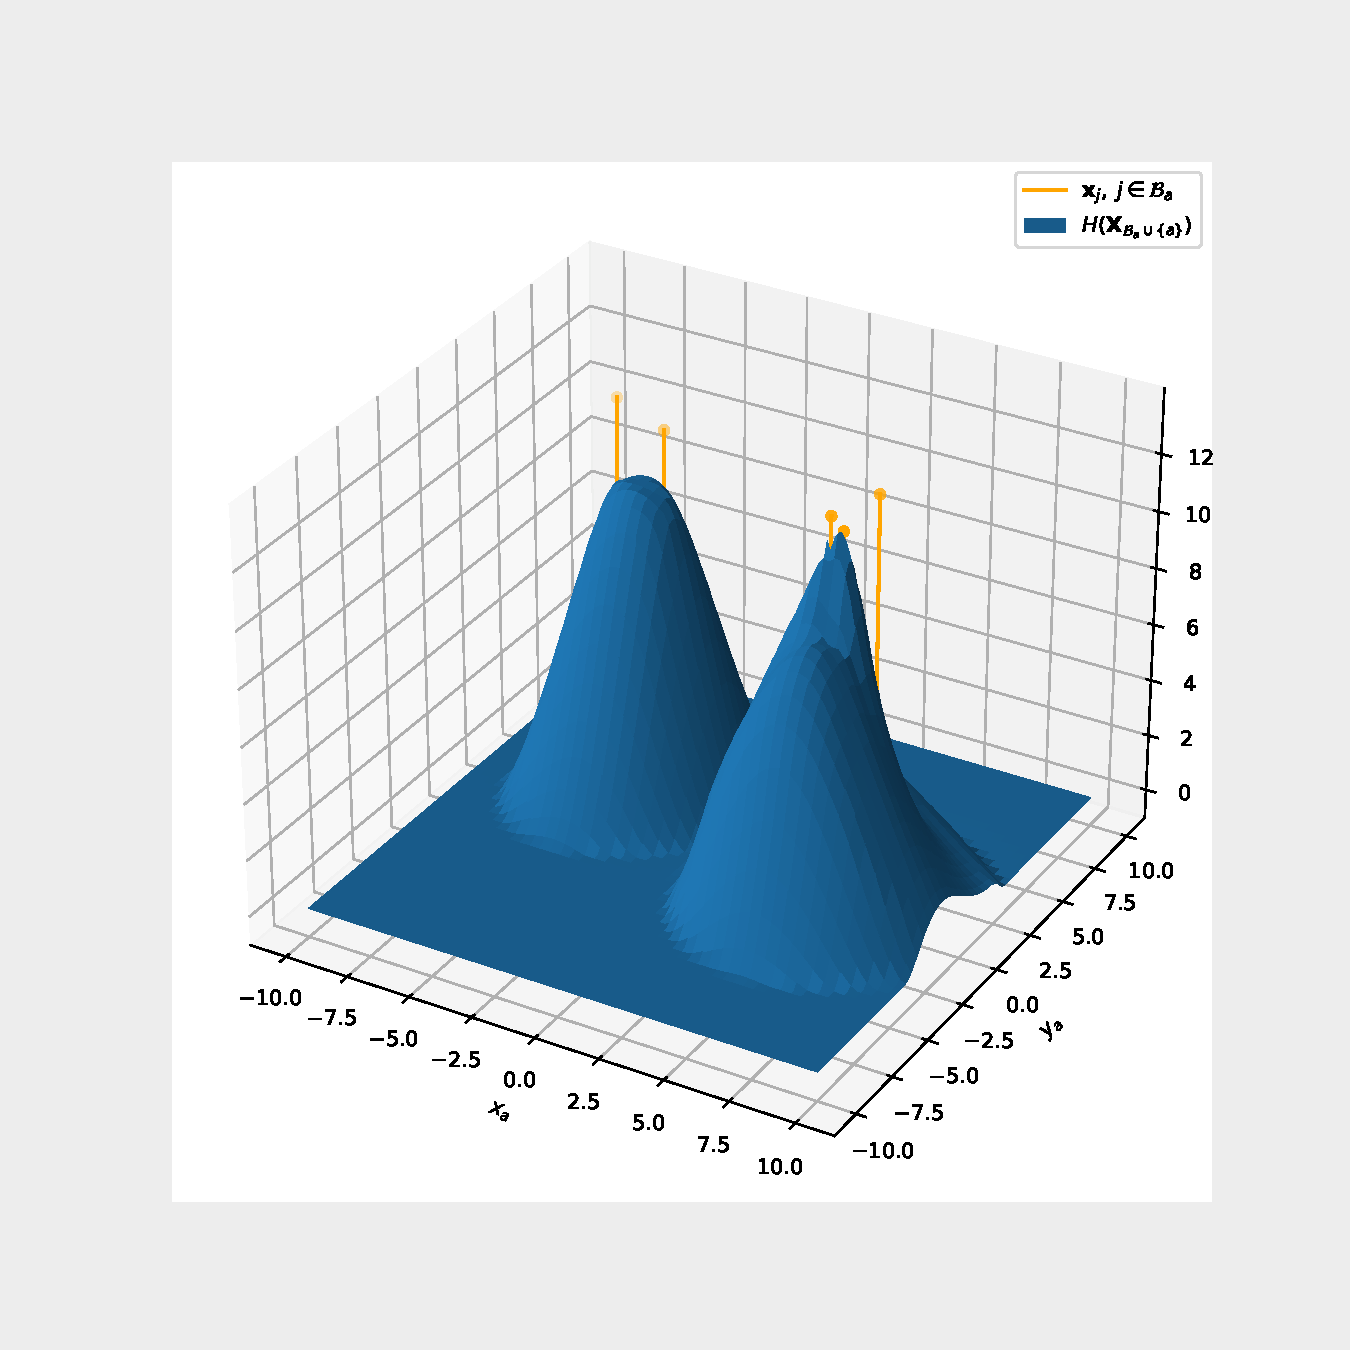
\includegraphics[width = .8\textwidth]{figs/objective_example.pdf}
  \caption{Objective function in \eqref{totally_objective} for agent $a$ with $|B_{a}| = 5$.}
  \label[fig]{objective_example}
\end{figure}